\chapter{Basis and related work} \label{computer vision}
    In this section, we introduce applications of deep learning on acoustic data. First the work this thesis uses as a basis, and then we describe some recent developments.
    
%\subsection{Applications of CV methods on acoustic data} \label{applications of computer vision}

%\section{Applications of Deep Learning in Acoustic Target Classification}

\section{Acoustic classification in multifrequency echosounder data using
deep convolutional neural networks} \label{unet_paper_acoustic}
    
        \begin{figure}[H]
        \centering
        %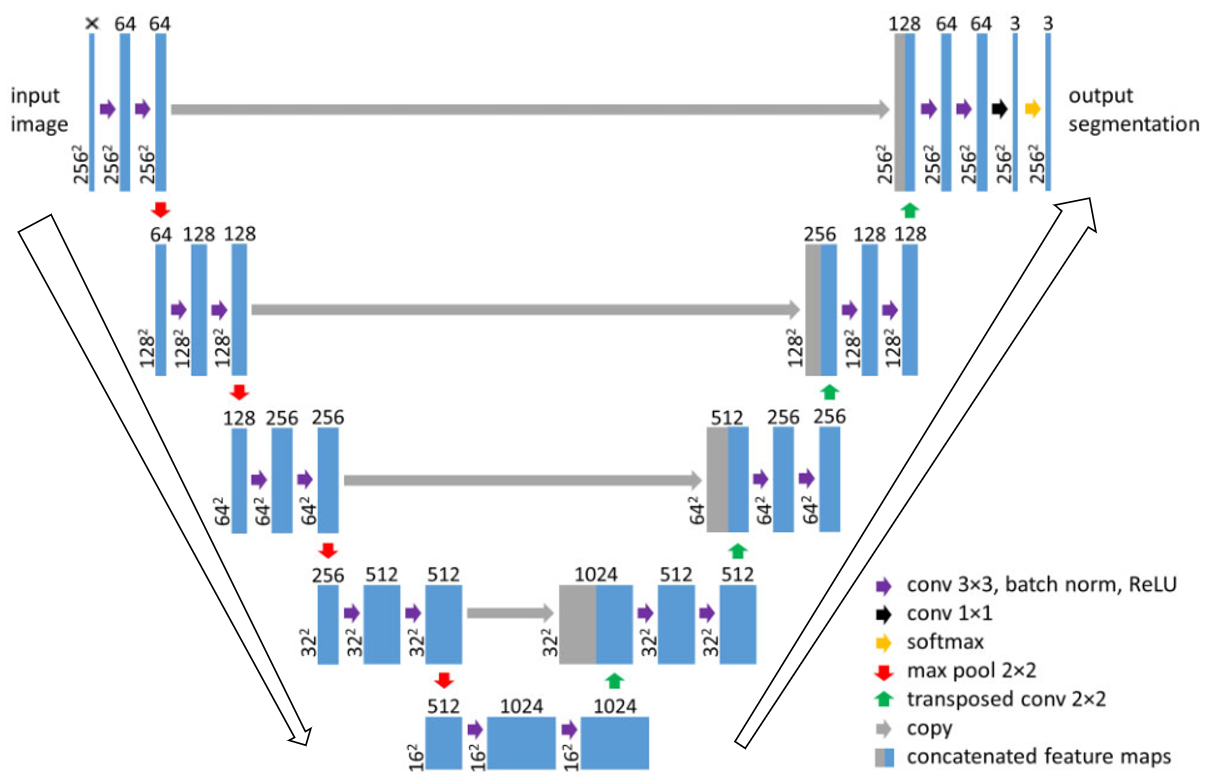
\includegraphics[scale=0.5]{figures/unet_arrows.png}
        \includesvg[inkscapelatex=false,width=1.0\textwidth,keepaspectratio]{figures/unet_brautset.svg}
        \caption[U-Net architecture]{U-Net architecture, the downwards facing arrow illustrates the contracting path and the one facing upwards is the expanding path. The color gets darker as the channels increase.}
      	\medskip 
        \label{unet__brautset_fig}
        \hspace*{15pt}\hbox{\scriptsize Credit: \citeauthor{brautaset2020acoustic}\cite{brautaset2020acoustic}}
    \end{figure}
    
    
    \citeauthor{brautaset2020acoustic}\cite{brautaset2020acoustic} had as objective to propose a deep learning method to classify and segment multi-frequency acoustic data gathered during acoustic trawl surveys, without using predefined features. Their work is the basis for the work contained in this thesis. Their architecture is visualized in figure \ref{unet__brautset_fig}, and the difference from the original U-Net implementation is the use of \textit{same convolutions} and \textit{batch normalization}. Furthermore, as the resolution of the layers in the contracting and expanding path has the same size, hence when concatenating, cropping is no longer needed. 
    
    \subsubsection{The Data}
    The data used originated from the yearly \textit{Norwegian North Sea Sandeel} acoustic trawl mission spanning 2007-2018. 2011-2016 was set as training and validation data, and 2007-2010 combined with 2017-2018 as test data. For all years, the \gls{lsss} system was used to categorize and annotate the data. The frequency channels extracted from each year were 18kHz, 38kHz, 70kHz and 200kHz. Operator annotations initially contained the classes \textit{sandeel}, \textit{other}, \textit{0-group sandeel} and \textit{possible sandeel}, and were annotated by the same operator. 0-group sandeel and possible sandeel were added to a new class \textit{ignore}, as both of them were edge cases which originated from an extraordinary event seen during a trawl or operator uncertainty. The annotations were converted to a pixel map of the same size as the \gls{sv} data, and all pixels not allocated to a class were set as the \textit{background class}. Annotations were originally designed to summarize the \gls{sv} values over an area, to estimate quantity. Hence, they were usually unrealistically square in shape, and larger than the actual school of fish. This is not suitable as labels for a \gls{cnn} as pixels around the edges in the annotations sometimes belonged to the wrong class. As a result, the annotations were approximately reshaped to be more similar to real schools of fish. The outline of the training methods applied is described in the methodology chapter (\textit{chapter \ref{methods}}) as it is heavily based on this article\cite{brautaset2020acoustic}.
    
    \subsubsection{Performance}
    They measured performance using two different methods\cite{brautaset2020acoustic}. The first method was to measure the performance over \textit{entire echograms} and all its pixels. While the second method extracted predictions in \textit{small regions} around existing annotations, and was applied due to  the observations of many schools missing their annotations. This would likely result in the decrease of many false positives being produced by the model, and would likely better reflect its actual performance. To have a benchmark to compare to, they used the traditional pipeline developed by \citet{korneliussen2016acoustic} which use an acoustic feature library to identify species, which do not use machine learning methods. The metric used was F1-score, where \textit{sandeel} was the \textit{positive}   while \textit{other} and \textit{background} was the \textit{negative}. 
    
    Small regions resulted in an overall F1-score of 0.87 for their model on all the test data after a threshold of 0.8 was applied to the probabilities, while the benchmark achieved a F1 score of 0.77. When applying the model to entire echograms, the performance decreased and ranged from 0.11-0.78 on individual test years. This was also mirrored by the benchmark method, which achieved 0.03-0.62. The decrease in performance over entire echograms was attributed to missing annotations, and many unidentified features in the data being allocated to the \textit{background} class. The latter would likely cause issues as their training scheme (\textit{described in section \ref{Data_loading_scheme_table}}) seldom focused on the background class. Data quality varied between different years due to changing weather conditions, fish populations and stages of development in software used during annotations. The model was concluded as able to reliably classify acoustic multifrequency measurements\cite{brautaset2020acoustic}.

%The training scheme later described in section \ref{Experiment settings} did not take many of these into account.

%\subsection{Applications of Deep Learning in Acoustic Target Classification}
\section{Related work}
In \citeyear{korneliussen2018acoustic} \citet{korneliussen2018acoustic} reported the most recent methods used for acoustic target classification. The mentioned methods applying \gls{ann}s, and were most frequently applied to single frequency channel data. Due to these being used in a supervised setting, they stressed the importance of high-quality annotations. Similar to the work detailed earlier in \citet{brautaset2020acoustic}, we will describe some newer research applying using deep learning to acoustic data.
   
\citet{marques2021detecting} compared different machine learning methods for automatically interpreting multi-frequency echograms, and proposed that a deep learning based end-to-end framework was best suited for the task. Their experiments handled the generation of square bounding boxes around schools of fish, and their results were comparable or better than those produced by human operators. The work was later extended with instance segmentation capabilities in \citeyear{marques2021instance}\cite{marques2021instance}. This produced more accurate predictions with pixel precision, and they described this as more befitting biological analysis.
 
\citet{semtantic-segm2021choi} proposed in \citeyear{semtantic-segm2021choi} a semi-supervised deep\footnote{A machine learning approach where you utilize both labeled and unlabeled data\cite{Goodfellow-et-al-2016}} learning network, with the intent of solving the reliance supervised \gls{ann}s have on the correct manual annotation of the acoustic data. By using the same data as \citet{brautaset2020acoustic}, they utilized \textit{two} loss functions which in alternating order optimize the same \gls{cnn}. This \gls{cnn} was based on an \gls{cnn} architecture called VGG-16\cite{simonyan2014very}. The first loss function seeks to \textit{cluster} the data by finding intrinsic characteristics in the data. The second loss function uses classification based on the existing annotated data. They showed that their model could outperform other traditional machine learning algorithms, both with or without missing annotations. Showing that we can efficiently process acoustic data with only a few annotated samples.





%        
%    \end{itemize}

% Setting the stage for the machine intelligence era in
% marine science - Cigdem Beyan et al.
%  - nevner brautaset, ikke noe mer innen acoustic categorization
%  - 








        
        
        
        
        

        
        
        
        
        
        
        %\citeauthor{VERFUSS201917} \citeyear{VERFUSS201917}\cite{VERFUSS201917} reviewed the current status of the unmanned vehicles, in combinations with a variety of sensors, used to monitor marine fauna. They discussed the different aspects to be considered when selecting systems in the context of a task. The task specifies the technical requirements of the vehicle, and this again what information will be gain. Regarding population monitoring tasks, which is the focus of this thesis, they stated that it is especially important that this information enables us to assign recorded animals to the correct species. Signifying the importance of developing methods to correctly classify species, and those that already exists may only work in the environment for which they were created. The market can today provide commercial systems within this field and enables affordable products and increase availability. They emphasized that unmanned vehicles have the potential to improve mission safety, and measurements while decreasing costs. Although, at the same time, may increase the need for more support vessels and additional personnel with expertise system knowledge.
 


        
        
        %- Measure the ipopulation, mitigation, and focal animal monitoringmpact of underwater sound on marine animals we focus on population monitoring
        %- population, mitigation, and focal animal monitoring
       % - unnmaned systems "
%The various methods require different information to be recorded
%about detected animals, which will determine what specific sensors are
%required for a given platform. Identification of animals to species or
%species group level is essential for all methods.
 %       - The system needs to be tailored to the spesific task
 %       - Developed to commercial use, arial, surface/under surface vessels
 %       - Systems that classify marine animals only works in the context in which they weree created
 %       -~18 kHz through to ~500 kHz.
 %       - smaller platform, less nois
 %       - low power means mor suceptible to currents and weather effects
 %       - In the case of self-powered platforms, it may be that
%the extended survey duration is a suitable trade-off for some disruption
%to the planned survey
 %       -  However, despite these additional
%considerations, autonomous vehicles' long deployment durations pre-
%sent a major advantage for marine animal surveys and their ability to
%move efficiently to other study areas make them a powerful asset.



%    - goal, (i) develop a deep learning
%        strategy that is suitable
%        for segmenting and classifying echosounder data collected during acoustic trawl surveys %without prior feature extraction; (ii) demonstrate that the strategy devel-
%        oped in (i) works on a real test case, and (iii) provide perspec- tives, e.g. pros and %cons, on the use of deep learning algorithms in the classification of acoustic %observations into acoustic catego-ries (e.g. species groups).
% - modified architecture, same convs, batch norm
% - trawl missions from 2007 - 2018, many classes, combined into three
% - four frequencies used -> output segmantation map of sandeel, other and background
% - preprocessing of the data, as we use the same approach this is described in the %AC-tool.
%    - regrid to 200kHz
% - modified the annotations to be more similar to actual schools of sandeel
% - balanced sampling 256x256x4 crops with regard to the information contained in the crop % equal probability from the dataset
% - a word about the classes.
% - a thing about the annotations, not deemed fully compatible with semantic segmentation, one %ator
%- Performance
%    - Training scheme outlined in the methodology, 
%    - stained by domain knowledge, and there could be more imacting performance
%        - when calculating F1 score, compare only examined regions withing 20 pixels of an actual annoation (false positive)
%        - 0.87 F1 at discriminate between sandeel (positive) and background and other as negative across the test data. Benchmark method got 0.77.
%        
%    - When evaluating entire echograms, was deem satisfactory for 2018 and 2017 at 0.78 and 0.68, benchmark (0.62 and 0.32)
%    - Both on complete echograms,unet (0.11 - 0.68) and 0.03-0.5)
%
%Echograms contain (problems): 
%- missing annotations, will confuse a pixel based classifier as there were clear signs of sandeel
%- false positives near the surface as, and was speculated to be dense layers of plankton, resulting in high sv values hence being classified as sandeel, and was missed was not data the model had been exposed to earlier. (this causes my model to likely classify this as sandeel). The exact plankton "Phaeocystis" produces gases which have high intensity at 18 and 38kHz, and could be a reason why the. The backround class contains everything not related to the other and sandeel class so will maybe contain other noise inducing factors, as seen when trying to predict entire echograms  
%
%- large uncertainy across years, weather conditions and school populations,  which affects %the quality quality of labeling. Historical data was affected by tools being under %development.
    
    
    
    
    
    
    %OBS! Må ha forklart U-net, accoustic klassifikasjon, F1 OBS, feature construction, statistical and machine learning methods!
    
    %To help assess the size of legal fishing quotas, acoustic trawls surveys are initiated to gather data. Before the data is of use, an operator manually needs to interpret the data in a time-consuming process to assign the acoustic back scattering to the correct category, but in turn often introduces bias. Several methods have been implemented to reduce this bias and with a goal to automate the process, but they all have a common weakness where they need a predefined feature space.  In 2020 a group of researchers implemented a U-net deep learning model to the problem and as this is an \gls{cnn} it does not need to have pre-designed features but learn them from the data. Sandeel  ~\cite{brautaset2020acoustic}. 
    
    %In this thesis, this will be a semantic segmentation of the classes \textit{background}, \textit{other } and most importantly \textit{sandeel}.
    
    
    
    %The \gls{crimac} used this model in their project (described in \ref{unet_paper_acoustic}) and had to do some small modifications to the network to fit their task. This modified U-Net is the one presented in this section, as this is the one used in the experiments. The core functionality of the network stays true to the original Unet, and the alterations done to the original will be explained later in this section.
    
    
    
    
    %Minor changes were made to adapt\citeauthor{unet_ronneberger2015}s original U-Net to the acoustic data used in \ref{unet_paper_acoustic}, as the input now had the form 4 x 256 x 256. The four channels being the frequencies used. The convolutions were set to \textit{same} instead of \textit{valid}, as were the original setting. This was done to make the size of the input and output match. Further, batch normalization was added to each convolution. 
    
 
 
 

%    @article{Marques2021InstanceSI,
%  title={Instance Segmentation-based Identification of Pelagic Species in Acoustic Backscatter Data},
%  author={Tunai Porto Marques and Melissa Cote and Alireza Rezvanifar and Alexandra Branzan Albu and Kaan %Ersahin and Todd Mudge and St{\'e}phane Gauthier},
%  journal={2021 IEEE/CVF Conference on Computer Vision and Pattern Recognition Workshops (CVPRW)},
%  year={2021},
%  pages={4373-4382}
%}
%- instance segmentation
%- automate the process, automatic bilogical analysis


    

    
    

    


        

    
    





%\chapter{Related Work}
%This chapter will start with a description of a deep learning architecture called U-Net, and %then an implementation of this network on acoustic data. The latter is the work this thesis %is heavily based upon. In the final part of this chapter, the context of the research field %will be described, focusing on deep learning and unmanned vehicles withing marine science.

%\section{Acoustic Classification In Multifrequency Echosounder Data Using Deep Convolutional %Neural Networks} \label{unet_paper_acoustic}
%    
%        \begin{figure}[H]
%        \centering
%        %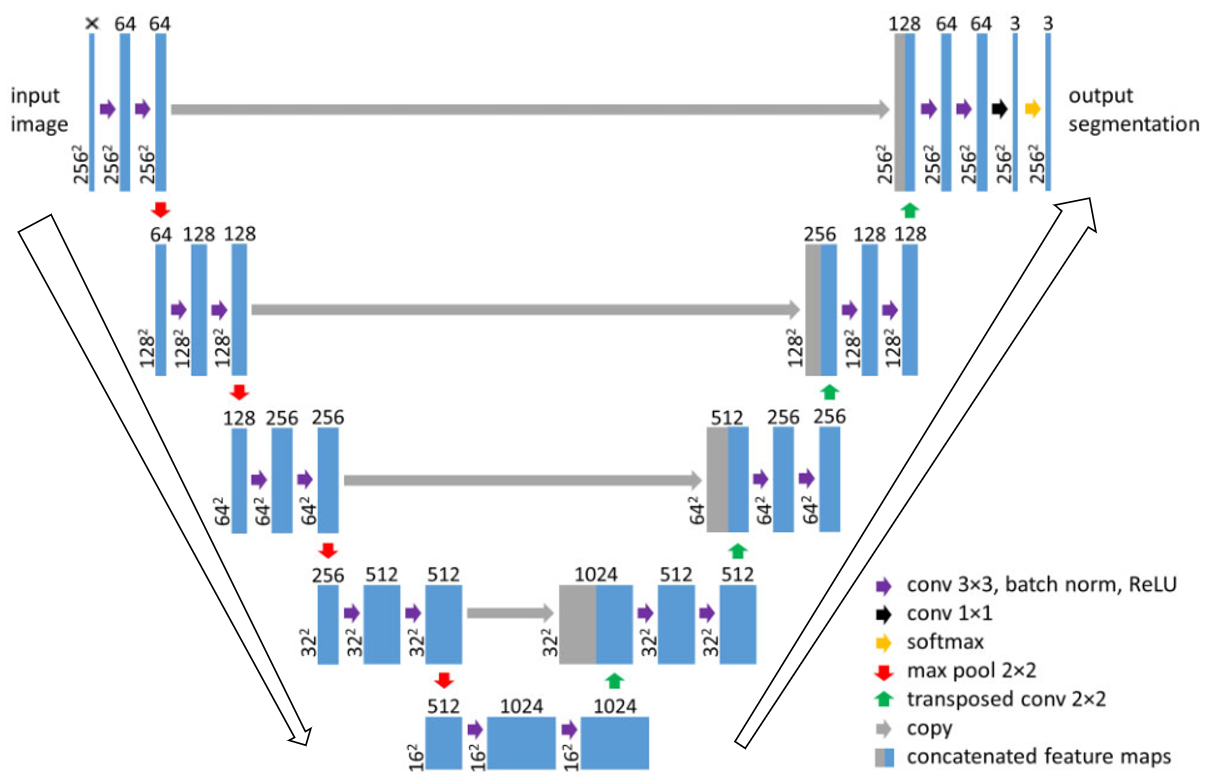
\includegraphics[scale=0.5]{figures/unet_arrows.png}
%        \includesvg[inkscapelatex=false,width=1.0\textwidth,keepaspectratio]{figures/unet_bra%utset.svg}
%        \caption[U-Net architecture]{U-Net architecture, the downwards facing arrow %illustrates the contracting path and the one facing upwards is the expanding path. %The color gets darker as the channels increase.}
%      	\medskip 
%        \label{unet__brautset_fig}
%        \hspace*{15pt}\hbox{\scriptsize Credit: %\citeauthor{brautaset2020acoustic}\cite{brautaset2020acoustic}}
%    \end{figure}
%    
%    
%    \citeauthor{brautaset2020acoustic}\cite{brautaset2020acoustic} had as objective to %propose a deep learning method to classify and segment acoustic data gathered during %acoustic trawl surveys, without using predefined features. This work is the backbone of %this thesis and the data is the same or very similar, hence a more detailed description %is provided. The acoustic data from the surveys are used as support when fisheries %estimate the allowed catches of different fish populations, and in this case %\textit{sandeel}. To estimate the quantity of fish, there is a linear relationship %between the \gls{sv} value and quantity as long as the correct species can be assigned to %the value. Today, the process of designating \gls{sv} to the proper species is heavily %influenced by human operators using a variety of tools, and trawl samples (biological %samples) \cite{korneliussen2016acoustic}. These tools use predefined features, and are %subject to not fit all situations equally well. 
%    
%    The deep learning architecture proposed was based on an altered version of %\citeauthor{unet_ronneberger2015}\cite{unet_ronneberger2015} %U-Net\cite{brautaset2020acoustic}. It is visualized in figure \ref{unet__brautset_fig}, %and the difference is the use of \textit{same convolutions} and \textit{batch %normalization}. Furthermore, as the resolution of the layers in the contracting and %expanding path had the same size, when concatenating, cropping was no longer needed. 
%    
%    The data used by this work and in this thesis originated from the yearly %\textit{Norwegian North Sea Sandeel} acoustic trawl mission spanning %2007-2018\cite{brautaset2020acoustic}. They quantify the stock of lesser sandeel %(\textit{Ammodytes marinus}), from now on, just \textit{sandeel}. 2011-2016 was set as %training and validation data, and 2007-2010 combined with 2017-2018 as test data. For all %years, the \gls{lsss} system was used to categorize and annotate the data. The frequency %channels extracted from each year was the 18kHz, 38kHz, 70kHz and 200kHz. Operator %annotations initially contained the classes \textit{sandeel}, \textit{other}, %\textit{0-group sandeel} and \textit{possible sandeel}, and were annotated by the same %operator. \textit{0-group sandeel} and \textit{possible sandeel} was added to a new class %\textit{ignore}, as both of them were edge cases, originated from an extraordinary event %seen during a trawl or operator uncertainty. The annotations were converted to a pixel %map of the same size as the \gls{sv} data (the output from the echosounder), and all %pixels not allocated to a class was set as the \textit{background class}. Annotations %were originally designed to summarize the \gls{sv} values over an area, to estimate %quantity. Hence, they were usually square and larger than the actual school of fish, and %not suitable as labels for a \gls{cnn} as pixels around the edges sometimes belonged to %the \textit{background class}. As a result, the annotations were approximately reshaped %to be more similar to real schools of fish. The outline of further methods applied is %described in the methodology chapter (chapter \ref{methods}) as it is based on this %article.
%    
%    Performance was measured using two different methods\cite{brautaset2020acoustic}. The %first method extracted predictions in \textit{small regions} around existing annotations, %and was applied due to  the observations of many schools lacking annotations. This would %likely result in the decrease of many false positives being produced by the model, and %would now reflect its actual performance. The second method was to measure the %performance over \textit{entire echograms}. To have a benchmark to compare to, they used %the pipeline developed by \citet{korneliussen2016acoustic} which use an acoustic feature %library to identify species. The metric used was F1-score, where \textit{sandeel} was the %\textit{positive}   while \textit{other} and \textit{background} was the %\textit{negative}. \textit{Small regions} resulted in an overall F1-score of 0.87 on all %the test data after a threshold of 0.8 was applied to the probabilities, while the %benchmark achieved a F1 score of 0.77. When applying the model to \textit{entire %echograms}, the performance decreased and ranged from 0.11-0.68 on individual test years. %This was also mirrored by the benchmark method, which achieved 0.03-0.50. The decrease in %performance over entire echograms was attributed to missing annotations, and many %unidentified features in the data being allocated to the \textit{background} class. The %training scheme later described in section \ref{Experiment settings} did not take many of %these into account. The quality of the data from different years varied due to different %weather conditions, fish populations and stages of development in software used during %annotations. The model was concluded as able to be reliably trained to classify acoustic %multifrequency measurements\cite{brautaset2020acoustic}.
%    
%\section{Deep Learning and Acoustic Target Classification}
%In \citeyear{korneliussen2018acoustic} \citet{korneliussen2018acoustic} reported the then %most recent methods used for acoustic target classification. The mentioned methods applying %\gls{ann}s all utilized the supervised learning approach, and were most frequently applied to %single frequency channel data. Due to the supervised setting, they stressed the importance of %high-quality annotations. Including the work detailed earlier in %\citet{brautaset2020acoustic}, we will describe some newer research in this section.
%   
%\citet{marques2021detecting} compared different machine learning methods for automatically %interpreting multi-frequency echograms, and proposed that a deep learning based end-to-end %framework was best suited for the task. Their experiments handled the generation of square %bounding boxes around schools of fish, and their results were comparable or better than those %produced by human operators. The work was later improved upon by applying an instance %segmentation method in \citeyear{marques2021instance}\cite{marques2021instance}. This %produced more accurate predictions with pixel precision, and they described this as more %befitting biological analysis.
% 
%\citet{semtantic-segm2021choi} proposed in \citeyear{semtantic-segm2021choi} a %semi-supervised deep learning network, with the intent of solving the reliance supervised %\gls{ann}s have on the correct manual annotation of the acoustic data. By using the same data %as \citet{brautaset2020acoustic}, they utilized \textit{two} loss functions which in %alternating order optimize the same \gls{cnn}. This \gls{cnn} was based on an \gls{cnn} %architecture called VGG-16\cite{simonyan2014very}. The first loss function seeks to %\textit{cluster} the data by finding intrinsic characteristics in the data. The second loss %function uses classification based on the existing annotated data. This combined use of loss %functions was, presumably, the first application to acoustic data. They showed that their %model could outperform other traditional machine learning algorithms, both with or without %missing annotations. Proving that we can efficiently process data with only a few annotated %samples.
%
%
%\section{Accoustic Classification of Sandeel (ammodytes marinus)}
%
%https://academic.oup.com/icesjms/article/66/6/1100/694183?login=true 
%- Size-dependent frequency response of sandeel schools
%    - historically hard to identify because no swim-bladder
%    - 200kHz for schools, 18 og 38 for individ-classifying
%    - some work shows:
%        - some difficulty classify schools og sandeel at 38 and 120kHz
%        - combinations of Sv at 18, 38, 120, and 200 kHz can effectively identify schools of %sandeel vs. mackerel and herring
%    - goal
%        - The objective of this study was to identify and exploit differences in frequency %responses to classify sizes of sandeel in schools.
%    - method in works:
%        - 18, 38, 120, and 200 kHz - further details in paper
%        - The borders of the schools were delineated in the 200-kHz echogram, because the Sv %from sandeel is strongest and the reverberant noise from gas-bearing phytoplankton is %lowest at this frequency. Catch and multi-f class for identification.
%        - To compare the frequency responses of each school, the sA measured at i frequencies %(f) were normalized by the mean sA for the four values of f, resulting in %proportional frequency responses [r(f)] -> 10 * log-scaled
%        - Changes in fish behaviour could change their R(f) values at 120 and 200 kHz, %possibly affecting the classification rate
%        - In the shallow water characteristic of the sandeel grounds, the sampling width of %the echosounder beam is small compared with the width of the trawl. Therefore, there %is a high probability of a mismatch between trawl catches and acoustic observations %for small schools in proximity to each other
%        -There was a significant size-dependent difference in the normalized frequency %response of schools comprising small, 1-year-old, and large, 2-year-old 
%        - proportional frequency responses [R(f)] at 18, 38, 120, and 200 kHz as independent %variables.
%%    \begin{itemize}
%%        \item ~Deep learning acoustic data
%%        \item litt historie kanskje 
%%        \item 2021 model, instance segmentation
%%        
%%        \item X Johnsen autonomous vessels
%%        \item Best frequency - 200kHz, and others
%%        \item X A review of unmanned vehicles for the detection and monitoring of marine %%fauna
%%        
%%    \end{itemize}
%
%% Setting the stage for the machine intelligence era in
%% marine science - Cigdem Beyan et al.
%%  - nevner brautaset, ikke noe mer innen acoustic categorization
%%  - 
%
%
%
%
%\section{Unmanned Vehicles in Marine Science}
%        In \citeyear{VERFUSS201917} \citeauthor{VERFUSS201917}\cite{VERFUSS201917} reviewed %the current status of systems consisting of unmanned vehicles and  sensors monitoring %marine life. The vehicles can operate stationary or moving, on the ocean surface, as %aerial or submerged.  They can both be remotely controlled, autonomous or a %combination. In the case of the acoustic sensors, they emphasized the need to be able %to efficiently assign the correct species to the measured animal. This directly %impacts the technical requirements of the vehicles purchased, as they need a minimum %amount of information provided by the sensors to solve the given task. Possibly, %further increasing the need for more support vessels and personnel with expertise %system knowledge. Many of the systems reviewed are commercially available, leading to %a growth in number and use. \citet{malde2020machine} states that this increase in %unmanned vehicles, combined with the possibility to gather more complex data, will %see an exponential increase in the data gathered in marine science. As a consequence, %increasing the need to make automated programs or better tools to aid in the current %manual data processing, which today is a major chokepoint. Furthermore, they state %that the nature of the data gathered will change, possibly in decreasing quality, as %humans will have less or no opportunities to actively engage in the information %gathering process that are autonomous. This means that unmanned surveys will have to %be planned in more detail. 
%        
%         During the summer of \citeyear{johnsen2020measuring} an unmanned vehicle was tested %in Årdalsfjorden in Norway and involved a kayak with an electric motor and only one %200kHz echosounder installed to measure \textit{sprat} %abundance\cite{johnsen2020measuring}. Results showed that the vehicle managed to %measure fish that usually live closer to the surface in the acoustic eight-meter %blind zone of the larger vessels, as the echosounders are usually installed on the %bottom part of the large research ship used during acoustic trawl surveys. In %addition, the vehicle produces significantly less noise in the water and are less %prone to scare away the fish. The lightweight kayak platform enabled it to collect %data from shallower water, earlier inaccessible to the larger vessels. The end %result was positive for the continued use of unmanned vehicles, but the manned %vessels are still needed for the biological samples in addition to the acoustic data %gathered. There was room for one more echosounder on the kayak, which could have %increased performance. Hence, which frequency to choose, in addition to the 200kHz, %relates to the question we seek to solve in this thesis.
%
%
%
%        
%        
%        
%        
%        
%
%        
%        
%        
%        
%        
%        
%        %\citeauthor{VERFUSS201917} \citeyear{VERFUSS201917}\cite{VERFUSS201917} reviewed the current status of the unmanned vehicles, in combinations with a variety of sensors, used to monitor marine fauna. They discussed the different aspects to be considered when selecting systems in the context of a task. The task specifies the technical requirements of the vehicle, and this again what information will be gain. Regarding population monitoring tasks, which is the focus of this thesis, they stated that it is especially important that this information enables us to assign recorded animals to the correct species. Signifying the importance of developing methods to correctly classify species, and those that already exists may only work in the environment for which they were created. The market can today provide commercial systems within this field and enables affordable products and increase availability. They emphasized that unmanned vehicles have the potential to improve mission safety, and measurements while decreasing costs. Although, at the same time, may increase the need for more support vessels and additional personnel with expertise system knowledge.
 


        
        
        %- Measure the ipopulation, mitigation, and focal animal monitoringmpact of underwater sound on marine animals we focus on population monitoring
        %- population, mitigation, and focal animal monitoring
       % - unnmaned systems "
%The various methods require different information to be recorded
%about detected animals, which will determine what specific sensors are
%required for a given platform. Identification of animals to species or
%species group level is essential for all methods.
 %       - The system needs to be tailored to the spesific task
 %       - Developed to commercial use, arial, surface/under surface vessels
 %       - Systems that classify marine animals only works in the context in which they weree created
 %       -~18 kHz through to ~500 kHz.
 %       - smaller platform, less nois
 %       - low power means mor suceptible to currents and weather effects
 %       - In the case of self-powered platforms, it may be that
%the extended survey duration is a suitable trade-off for some disruption
%to the planned survey
 %       -  However, despite these additional
%considerations, autonomous vehicles' long deployment durations pre-
%sent a major advantage for marine animal surveys and their ability to
%move efficiently to other study areas make them a powerful asset.



%    - goal, (i) develop a deep learning
%        strategy that is suitable
%        for segmenting and classifying echosounder data collected during acoustic trawl surveys %without prior feature extraction; (ii) demonstrate that the strategy devel-
%        oped in (i) works on a real test case, and (iii) provide perspec- tives, e.g. pros and %cons, on the use of deep learning algorithms in the classification of acoustic %observations into acoustic catego-ries (e.g. species groups).
% - modified architecture, same convs, batch norm
% - trawl missions from 2007 - 2018, many classes, combined into three
% - four frequencies used -> output segmantation map of sandeel, other and background
% - preprocessing of the data, as we use the same approach this is described in the %AC-tool.
%    - regrid to 200kHz
% - modified the annotations to be more similar to actual schools of sandeel
% - balanced sampling 256x256x4 crops with regard to the information contained in the crop % equal probability from the dataset
% - a word about the classes.
% - a thing about the annotations, not deemed fully compatible with semantic segmentation, one %ator
%- Performance
%    - Training scheme outlined in the methodology, 
%    - stained by domain knowledge, and there could be more imacting performance
%        - when calculating F1 score, compare only examined regions withing 20 pixels of an actual annoation (false positive)
%        - 0.87 F1 at discriminate between sandeel (positive) and background and other as negative across the test data. Benchmark method got 0.77.
%        
%    - When evaluating entire echograms, was deem satisfactory for 2018 and 2017 at 0.78 and 0.68, benchmark (0.62 and 0.32)
%    - Both on complete echograms,unet (0.11 - 0.68) and 0.03-0.5)
%
%Echograms contain (problems): 
%- missing annotations, will confuse a pixel based classifier as there were clear signs of sandeel
%- false positives near the surface as, and was speculated to be dense layers of plankton, resulting in high sv values hence being classified as sandeel, and was missed was not data the model had been exposed to earlier. (this causes my model to likely classify this as sandeel). The exact plankton "Phaeocystis" produces gases which have high intensity at 18 and 38kHz, and could be a reason why the. The backround class contains everything not related to the other and sandeel class so will maybe contain other noise inducing factors, as seen when trying to predict entire echograms  
%
%- large uncertainy across years, weather conditions and school populations,  which affects %the quality quality of labeling. Historical data was affected by tools being under %development.
    
    
    
    
    
    
    %OBS! Må ha forklart U-net, accoustic klassifikasjon, F1 OBS, feature construction, statistical and machine learning methods!
    
    %To help assess the size of legal fishing quotas, acoustic trawls surveys are initiated to gather data. Before the data is of use, an operator manually needs to interpret the data in a time-consuming process to assign the acoustic back scattering to the correct category, but in turn often introduces bias. Several methods have been implemented to reduce this bias and with a goal to automate the process, but they all have a common weakness where they need a predefined feature space.  In 2020 a group of researchers implemented a U-net deep learning model to the problem and as this is an \gls{cnn} it does not need to have pre-designed features but learn them from the data. Sandeel  ~\cite{brautaset2020acoustic}. 
    
    %In this thesis, this will be a semantic segmentation of the classes \textit{background}, \textit{other } and most importantly \textit{sandeel}.
    
    
    
    %The \gls{crimac} used this model in their project (described in \ref{unet_paper_acoustic}) and had to do some small modifications to the network to fit their task. This modified U-Net is the one presented in this section, as this is the one used in the experiments. The core functionality of the network stays true to the original Unet, and the alterations done to the original will be explained later in this section.
    
    
    
    
    %Minor changes were made to adapt\citeauthor{unet_ronneberger2015}s original U-Net to the acoustic data used in \ref{unet_paper_acoustic}, as the input now had the form 4 x 256 x 256. The four channels being the frequencies used. The convolutions were set to \textit{same} instead of \textit{valid}, as were the original setting. This was done to make the size of the input and output match. Further, batch normalization was added to each convolution. 
    
 
 
 

%    @article{Marques2021InstanceSI,
%  title={Instance Segmentation-based Identification of Pelagic Species in Acoustic Backscatter Data},
%  author={Tunai Porto Marques and Melissa Cote and Alireza Rezvanifar and Alexandra Branzan Albu and Kaan %Ersahin and Todd Mudge and St{\'e}phane Gauthier},
%  journal={2021 IEEE/CVF Conference on Computer Vision and Pattern Recognition Workshops (CVPRW)},
%  year={2021},
%  pages={4373-4382}
%}
%- instance segmentation
%- automate the process, automatic bilogical analysis
%
%
%
%\section{Terminology of Multidimensional Arrays}
    %This chapter will frequently describe multidimensional arrays; therefore this section will clarify some  terms used in regard to multidimensional arrays in this thesis. Multidimensional arrays consist of multiple 2-dimensional arrays. These are called \textit{channels}, and have uniform \textit{resolution}. \textit{Depth} denotes the number of channels, while the resolution indicates the \textit{height} and \textit{width} of the channels. Thus, a multidimensional array can be described with \textit{height} x \textit{width} x \textit{depth}. The terms are illustrated in figure \ref{Multidimensional array terminology}.
    %
    %    \begin{figure}[H]
    %    \centering
    %                    \includesvg[inkscapelatex=false,width=0.8\textwidth,keepaspectratio]{figures/n_array_terminology.svg}
    %    \caption[Multidimensional  array]{Illustrations of the resolution (\textit{height} and \textit{width}), and \textit{depth} of a multidimensional array where the depth is split into \textit{channels} (different colors). In this example, the resolution is 3×3 and the depth is 4. }
    %  	\medskip 
    %    \label{Multidimensional array terminology}
    %\end{figure}